%% PG-GAT journal paper - Computer Vision and Image Understanding (Elsevier)
%% Template: CVIU bundle (paper_cviu/template/cviu), class options as shipped (D7):
%%   \documentclass[times,twocolumn,final,authoryear]{elsarticle} + ycviu.sty, model2-names.bst
%% Working agreement and decision log: docs/paper_cviu_guide.md. Sentence-per-line source.
%% Agent builds go to build_agent/ (see build.sh); never build in this directory.
\documentclass[times,twocolumn,final,authoryear]{elsarticle}
\usepackage{ycviu}

\usepackage{amsmath,amssymb}
\usepackage{booktabs}
% (placeins section barrier removed 2026-10-15: in two-column mode it flushes like a page break and left blank columns)
% Let tall column floats sit on a text page (rather than a float-only column, which the section barrier turns into a blank column).
\renewcommand{\topfraction}{0.9}
\renewcommand{\dbltopfraction}{0.9}
\renewcommand{\textfraction}{0.07}
\renewcommand{\floatpagefraction}{0.85}
\renewcommand{\dblfloatpagefraction}{0.85}
\usepackage{url}
\usepackage{xcolor}

\journal{Computer Vision and Image Understanding}

\begin{document}

\begin{frontmatter}

%% Title changed 2026-11-03: "skeleton-aware" dropped because of the name collision with skeleton-based action recognition (guide D15).
\title{Detector-independent keypoint grouping for multi-person pose estimation with a graph attention network}

\author[1]{Dean \snm{Mills}\corref{cor1}}
\cortext[cor1]{Corresponding author.}
\ead{deansmills@gmail.com}
\author[1]{Hans \snm{Grobler}}
\address[1]{Department of Electrical, Electronic and Computer Engineering, University of Pretoria, Pretoria, South Africa}

%% Journal-set dates; leave commented until acceptance.
%\received{}
%\finalform{}
%\accepted{}
%\availableonline{}
%\communicated{}

\begin{abstract}
Bottom-up multi-person pose estimators assign detected keypoints to people using a grouping mechanism trained jointly with the detector.
The grouping therefore cannot be reused once the detector changes.
This work treats grouping as a separate module and measures the cost of that separation.
The proposed grouping module, PG-GAT, is a graph attention network with a type-pair attention bias, skeleton-relative position encoding, and same-type repulsion heads; it embeds keypoints so that $k$-means recovers the people, and a head trained on the frozen embeddings estimates the person count.
Trained on synthetic scenes and fine-tuned on COCO, PG-GAT reaches a pose grouping accuracy of 0.9715 on annotated COCO validation keypoints and 0.9591 on HigherHRNet detections, against 0.9847 for the detector's jointly trained associative embedding on the same detections.
Applied without retraining to YOLO11x-pose and RTMO-L, the autonomous pipeline trails the native grouping of all three detectors by 0.020 to 0.022.
At the system level, the cost is 0.048 average precision on identical keypoints, rising to 0.076 in scenes with six or more people.
Learned grouping heads and modularity-based clustering tested here did not improve on $k$-means, whereas embedding changes produced gains that transfer to real data, identifying the embedding as the limiting component.

\end{abstract}

\begin{keyword}
%% Keyword count not stated by the Guide; the dissertation summary lists twelve, trimmed here to the MEng scope.
\KWD Multi-person pose grouping\sep Bottom-up pose estimation\sep Graph attention network\sep Detector independence\sep Synthetic-to-real transfer\sep Contrastive learning
\end{keyword}

\end{frontmatter}

\section{Introduction}
\label{sec:intro}

% Figure 1 is defined here, ahead of the text that cites it, so the two-column float lands at the top of page 2;
% defined later it was deferred past the section barrier (placeins) and left page 2 with an empty column.
\begin{figure*}[!t]
    \centering
    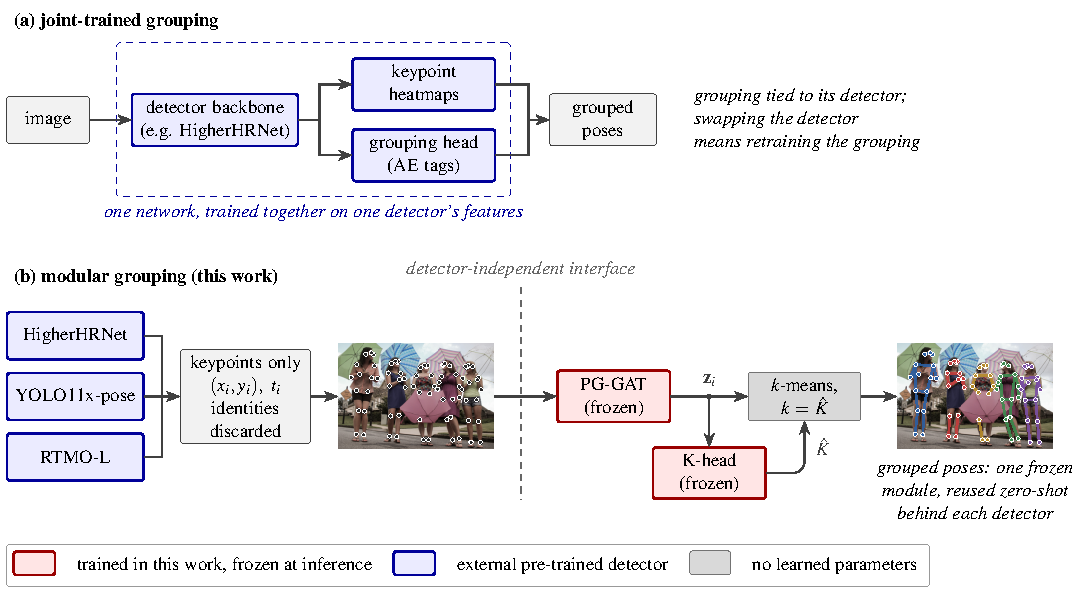
\includegraphics[width=\textwidth]{figures/concept_modular.pdf}
    \caption{Joint-trained versus modular grouping.
    (a) In established bottom-up methods the grouping head is trained with the keypoint detector
    on its internal features, which ties the grouping to that detector.
    (b) The modular pipeline exposes a keypoint-only interface shared by three detectors:
    PG-GAT embeds the detected keypoints, the K-head estimates the number of people $\hat K$,
    and $k$-means partitions the embeddings.
    PG-GAT and the K-head are trained once and remain frozen when the detector changes.
    Insets: COCO \texttt{val2017} image 281759 with the pooled HigherHRNet detections
    before grouping (grey) and after grouping by the modular pipeline (coloured by person).}
    \label{fig:concept}
\end{figure*}

% --- from chapter1_context.tex ---
In multi-person pose estimation, every person in an image must be localised at a fixed set of
anatomical joints, the seventeen joints of the COCO skeleton~\citep{lin2014coco}.
Bottom-up methods split the task into two stages:
a detector finds every keypoint in the image without assigning them to people,
and a grouping stage then assigns each detected keypoint to a person.
Keypoint detection is well studied,
and high-resolution convolutional backbones~\citep{sun2019hrnet,cheng2020higherhrnet},
transformer estimators~\citep{xu2022vitpose}
and human-centric foundation models~\citep{khirodkar2024sapiens} have raised localisation
accuracy on COCO to a point where further gains are small.
Grouping remains difficult for structural reasons.
The number of people is unknown at inference,
each person contributes at most one keypoint of each joint type,
occlusion and truncation remove keypoints without a predictable pattern,
and where people overlap in the image, same-type keypoints,
such as two left elbows, end up close together.

% --- from chapter1_context.tex and chapter1_research_gap.tex ---
In established bottom-up methods the grouping decision comes from a mechanism
trained jointly with the detector.
Part-affinity fields~\citep{cao2017openpose},
associative-embedding tags~\citep{newell2017associative,cheng2020higherhrnet},
centre-offset regression~\citep{geng2021dekr}
and end-to-end set prediction~\citep{shi2022petr} are the forms this mechanism takes,
and every one of them couples the grouping to a particular backbone.
The coupling buys accuracy at the cost of reuse: a grouping mechanism trained with one
detector cannot be detached and applied to the output of another.
The alternative, a grouping module that consumes keypoints from any detector,
has received comparatively little attention.
Among graph-based methods, hierarchical graph grouping~\citep{jin2020hgg} is trained jointly
with its detector,
and graph edge classification~\citep{maher2025gec} is detector-independent but classifies
pairs of keypoints rather than learning a representation of each keypoint.

This work develops the modular alternative and measures what the separation costs
(Figure~\ref{fig:concept}).
The interface between detector and grouping stage carries only detected keypoint
coordinates, visibility flags and joint types.
A graph attention network embeds the detected keypoints,
a small head, the K-head, estimates the number of people $\hat K$ from the embeddings,
and $k$-means partitions the embeddings into people.
The network and the head are trained once and remain frozen when the detector changes.
The accuracy lost to this separation is measured against a deliberately chosen
joint-trained reference:
the associative-embedding grouping of HigherHRNet~\citep{cheng2020higherhrnet},
evaluated on identical detections.
The same frozen module is then applied without retraining
to two further detectors from different architectural families.

% --- from chapter1_research_contributions.tex and summary.tex ---
The main contributions are as follows.
\begin{itemize}
    \item \textbf{PG-GAT}, a pose grouping graph attention network extending GATv2~\citep{brody2022gatv2}
    with a type-pair attention bias, skeleton-relative position encoding and same-type repulsion heads.
    It is trained on synthetic scenes and fine-tuned on COCO, and with a $k$-means read-out
    reaches 0.9715 pose grouping accuracy on COCO validation keypoints
    and 0.9591 on HigherHRNet detections, against 0.9847 for the detector's jointly trained
    associative embedding on the same detections.
    \item \textbf{Evidence that the embedding, not the grouping head, limits accuracy}: three learned
    grouping heads and ten modularity-based clustering variants did not improve on $k$-means
    once the model is applied to real data, while changes to the embedding produced gains
    that transfer to real data. Attention analysis shows that PG-GAT directs its attention along
    same-person skeletal edges and away from same-type edges.
    \item \textbf{A measured cost of modularity}: with the K-head trained on the frozen embeddings,
    the pipeline needs no ground truth at inference. Applied zero-shot to YOLO11x-pose~\citep{ultralytics2024yolo11}
    and RTMO-L~\citep{lu2024rtmo}, it trails the native grouping of all three detectors
    by 0.020 to 0.022 on matched detections.
    At the system level the cost is 0.048 AP on identical joints,
    rising to 0.076 in scenes with six or more people, beyond the synthetic training range.
    \item \textbf{Documented negative results}, in the configurations tested,
    for a hyperbolic embedding, a triplet-based graph primitive and appearance features,
    and the mechanism of failure in each case.
\end{itemize}
\section{Related work}
\label{sec:related}

\subsection{Bottom-up grouping and its coupling to the detector}
\label{sec:related_grouping}

% --- from chapter2_grouping.tex 2.2.1-2.2.4 ---
Most of the bottom-up grouping literature falls into four lineages.
In the first, OpenPose~\citep{cao2017openpose} predicts a part-affinity field for every limb alongside the keypoint
heatmaps, scores candidate joint pairs by the line integral of the field,
and assembles the skeletons one limb at a time by greedy bipartite matching;
PifPaf~\citep{kreiss2019pifpaf} refines the fields but keeps the greedy assembly.
In the second, associative embedding~\citep{newell2017associative} attaches a head that predicts a tag per keypoint,
each tag being pulled towards its person's mean and pushed away from other people's means,
and grouping is done by clustering the tags;
HigherHRNet~\citep{cheng2020higherhrnet} applies the mechanism to the high-resolution HRNet backbone~\citep{sun2019hrnet}.
In the third, PersonLab~\citep{papandreou2018personlab} regresses offsets between keypoints of the same person,
DEKR~\citep{geng2021dekr} regresses offsets from a person centre to its keypoints,
and CenterGroup~\citep{braso2021centergroup} associates keypoints with centres through transformer attention.
The fourth is set prediction: PETR~\citep{shi2022petr}, ED-Pose~\citep{yang2023edpose},
GroupPose~\citep{liu2023grouppose} and QueryPose~\citep{xiao2022querypose} follow DETR~\citep{carion2020detr}
and let each pose query predict a complete skeleton, with no separate grouping stage.
In all four lineages the grouping representation is learned jointly with the detector's features.
This joint training lets the grouping adapt to the detector's errors
and explains much of the accuracy these methods reach.
It also means that the grouping cannot be moved to another detector:
the fields, tags and offsets are tied to the backbone's resolution, stride and features,
and set prediction exposes no per-keypoint representation at all.

\subsection{Graph-based grouping and graph networks on pose}
\label{sec:related_graph}

% --- from chapter2_grouping.tex 2.2.5 and chapter2_gnn_pose.tex 2.3.1-2.3.4 ---
A smaller body of work approaches grouping as a graph problem.
Hierarchical graph grouping (HGG)~\citep{jin2020hgg} merges sub-graphs of detected keypoints with a learned discriminator,
but the graph and the merge predictor are trained jointly with the detector.
Yang et al.~\citep{yang2023instanceaware} supervise the self-attention of a vision transformer to encode person membership,
which places the grouping inside the detector backbone.
Graph edge classification (GEC)~\citep{maher2025gec} is the closest precedent to this work:
it operates on the output of an existing detector, predicts a same-person label for pairs of keypoints
and recovers people as connected components.
It is detector-independent, but it produces a binary decision per edge rather than a representation per keypoint.

Elsewhere in pose research, graph neural networks are used widely.
Skeleton-based action recognition builds spatial-temporal graphs over the joints of a single person~\citep{yan2018stgcn,shi2019twostreamadaptive},
and 3D lifting applies graph convolutions to one person's 2D skeleton~\citep{zhao2019semanticgcn,ci2019optimizing,liu2020gastnet}.
In both cases the keypoints are already grouped,
and the output is a label or coordinates, not an identity signal per keypoint.
The graph and clustering literature offers learned alternatives to a plain read-out:
deep embedded clustering~\citep{xie2016dec}, slot attention~\citep{locatello2020slotattention},
supervised graph partitioning from face clustering~\citep{yang2019face,yang2020gcnve},
and modularity maximisation~\citep{newman2006modularity} with its differentiable relaxation DMoN~\citep{tsitsulin2023dmon}.
This work evaluates these alternatives to the $k$-means read-out for keypoint grouping.

\subsection{Position of this work}
\label{sec:related_gap}

% --- from chapter2_gap.tex 2.6.1 ---
Detectors are now strong enough that grouping is the main remaining source of error in bottom-up systems,
yet every established grouping mechanism is tied to its detector.
Modular grouping on detached keypoints has a single detector-independent precedent,
and it classifies edges.
Graph networks on pose, by contrast, have been used almost entirely on keypoints that are already grouped.
No prior work in this modular setting trains a detector-independent graph network
that produces a per-keypoint embedding for multi-person grouping,
or estimates the number of people within the same pipeline.
\section{Method}
\label{sec:method}

% --- from chapter3_problem_formulation.tex (intro + 3.3.1) and chapter3_integration.tex (intro) ---
Multi-person pose grouping is treated in this work as a stage that follows keypoint detection and is independent of the detector.
A bottom-up keypoint detector produces a set of two-dimensional keypoint detections for the whole image,
each carrying one of the seventeen COCO joint types~\citep{lin2014coco}.
The grouping stage partitions those detections into person skeletons without access to the image or to the detector's
internal representation (Figure~\ref{fig:pipeline}); the only quantities that cross the interface between the detector
and the grouping module are the keypoint coordinates, the visibility flags and the joint types.
The detector can therefore be replaced without changing or retraining the grouping network, and this separation is the
central design choice of the work.
It departs from architectures in which detection and grouping are learned together,
such as associative embedding~\citep{newell2017associative}, DEKR~\citep{geng2021dekr}
and ED-Pose~\citep{yang2023edpose},
whose grouping mechanism is tied to the features of the detector it was trained with.

\begin{figure*}[!t]
    \centering
    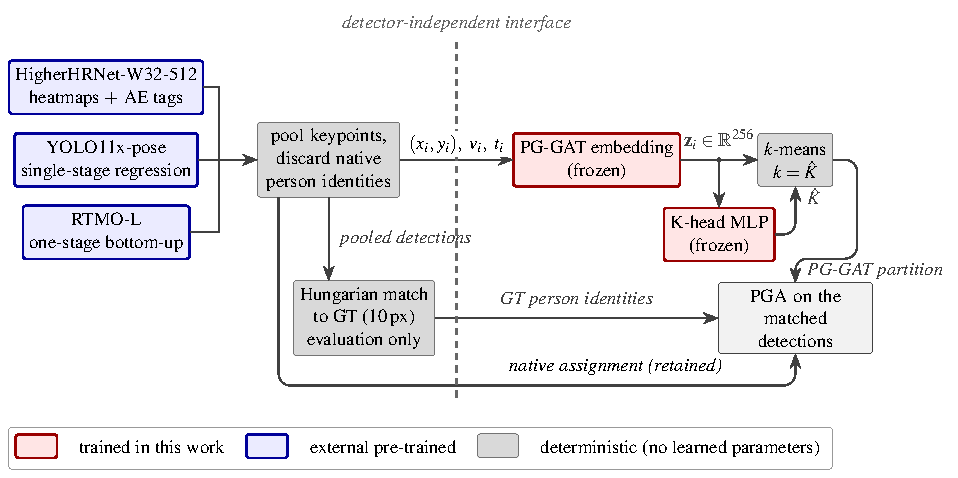
\includegraphics[width=\textwidth]{figures/e2e_interface.pdf}
    \caption{The detector-independent interface.
    Each detector produces a set of keypoint detections; its native person assignments are discarded,
    and only the keypoint coordinates, visibility flags and joint types cross the interface (dashed line).
    The frozen PG-GAT embeds the detections, the frozen K-head estimates the person count $\hat K$,
    and $k$-means produces the partition.
    Ground truth (GT) is used only for evaluation: detections are matched to the annotated keypoints,
    and both the PG-GAT partition and the detector's retained native assignment are scored on the matched set.}
    \label{fig:pipeline}
\end{figure*}

\subsection{Problem formulation}
\label{sec:method_problem}

% --- from chapter3_problem_formulation.tex 3.3.1 and 3.3.3 ---
For an image containing $K$ people, the detector produces $N$ keypoint detections, collected into the set
\begin{equation}
    \mathcal{X}
    = \bigl\{(\mathbf{p}_i, t_i, v_i)\bigr\}_{i=1}^{N},
    \label{eq:detections}
\end{equation}
where $\mathbf{p}_i \in [0,1]^2$ is the normalised image-plane position of detection $i$,
$t_i \in \mathcal{T} = \{1,\dots,T\}$ is its joint type with $T=17$ for COCO,
and $v_i$ is its visibility state.
The grouping task is to predict a labelling
\begin{equation}
    \hat{\mathbf{y}} \in \{1,\dots,K\}^{N},
    \label{eq:labelling}
\end{equation}
in which two detections share a label if and only if they belong to the same person.
Ground-truth assignments $\mathbf{y}^{\star}$ are available during training;
at inference the number of people $K$ is unknown and must be estimated from the detections themselves.

The problem is decomposed into three components.
An embedding network maps every detection to a vector $\mathbf{z}_i \in \mathbb{R}^{d}$ such that detections of the same
person lie close together and detections of different people lie apart.
A read-out recovers the person assignments from the embeddings, given $K$.
A person-count estimator supplies $K$ when no oracle value is available.
The embedding network carries the discriminative work, the read-out is deliberately kept simple,
and the count estimator is trained separately so that it cannot alter the embedding.

\subsection{Graph construction}
\label{sec:method_graph}

% --- from chapter3_problem_formulation.tex 3.3.2 and chapter3_dataset.tex (node features) ---
The detections of a single image form a graph $\mathcal{G} = (\mathcal{V}, \mathcal{E})$ with one node per detection,
$|\mathcal{V}| = N$.
The continuous node feature is
\begin{equation}
    \mathbf{x}_i
    =
    [\,x_{\text{norm}},\;
      y_{\text{norm}},\;
      v_{\text{norm}}\,]
    \in \mathbb{R}^{3},
    \label{eq:node_feature_no_depth}
\end{equation}
the image-plane position, normalised by the image size, and the visibility, scaled to $[0,1]$
(0.5 for an occluded and 1 for a visible annotated keypoint; every detected keypoint is treated as visible).
The input to the first layer of the embedding network combines this feature with a learned representation of the joint type,
\begin{equation}
    \mathbf{h}_i^{(0)}
    = \bigl[\,\mathbf{x}_i \,\big\|\,
    \mathrm{emb}_{\mathcal{T}}(t_i)\,\bigr]
    \in \mathbb{R}^{d_0},
    \label{eq:layer0_input}
\end{equation}
where $\mathrm{emb}_{\mathcal{T}} : \{1, \dots, T\} \to \mathbb{R}^{d_t}$ is a learnable lookup table over the joint types
and $d_t = 64$ in the final configuration.
Keeping the type embedding separate from the spatial features lets the network learn what a joint type means
independently of where it is detected.

Each node is connected to its $k$ nearest neighbours ($k$NN) in the image plane, with $k=16$ in the final configuration.
The edge set is directed and contains no self-loops, although the attention layers add one to every node;
an edge is reciprocated only when the two nodes each select the other.
The same $k$ is used for training and evaluation.
Two properties of this graph shape the method.
Its edges encode spatial proximity rather than identity:
two nearby keypoints are connected whether or not they belong to the same person,
and the left shoulders of two overlapping people can be neighbours although they must receive different labels.
The joint type of every node, on the other hand, is known,
and the network can therefore exploit the structure of the human skeleton without any further information from the detector.

\subsection{PG-GAT}
\label{sec:method_pggat}

% --- from chapter3_baseline.tex 3.5.1 (GATv2 rationale) and chapter3_pg_gat.tex (intuition + three modifications) ---
Message passing on $\mathcal{G}$ uses GATv2~\citep{brody2022gatv2}, the graph attention network (GAT) variant
in which the attention ranking of a node's neighbours depends on the query node.
The original GAT~\citep{velickovic2018gat} computes a static ranking shared by every query, which is limiting here:
a keypoint must treat a nearby joint of its own type differently from an anatomically related
joint of another type.
Standard GATv2 attention, however, does not distinguish between categories of edges;
the same mechanism processes a left-shoulder to left-elbow edge, a left-shoulder to right-shoulder edge
and a left-shoulder to right-ankle edge, although these relationships carry different evidence for grouping.
Two detections of the same joint type cannot belong to one person,
skeletally adjacent joint types are strong evidence that two detections belong together,
and pairs that are distant in both the image and the skeleton carry little.
The baseline for this work is a standard GATv2 embedding network
with two layers, four heads and a hidden dimension of 64, a 128-dimensional output,
a 32-dimensional joint-type embedding and a graph with $k=8$.
PG-GAT (pose grouping graph attention network) builds on this baseline with three modifications
that expose the differences between edge categories to the attention mechanism.
Each modification can be enabled independently, and the GATv2 operator is retained throughout;
the resulting layer is shown in Figure~\ref{fig:pggat}.

\begin{figure*}[!t]
    \centering
    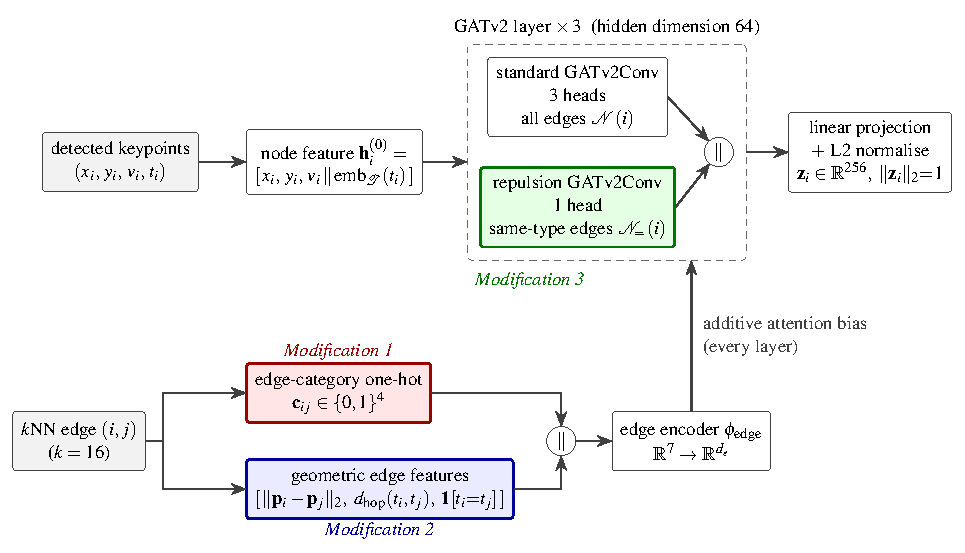
\includegraphics[width=\textwidth]{figures/pggat_architecture.pdf}
    \caption{The PG-GAT layer.
    The node feature contains the keypoint position, the visibility flag and a learned joint-type embedding.
    Modification~1 assigns every edge to one of four categories
    and supplies the one-hot category to the GATv2 attention through a learned additive bias (red).
    Modification~2 adds three geometric features to the edge representation: the Euclidean distance, the skeleton hop distance
    and a same-type indicator (blue).
    Modification~3 splits the multi-head attention into a standard sub-layer over the full neighbourhood
    and a repulsion sub-layer restricted to same-type edges (green).}
    \label{fig:pggat}
\end{figure*}

\paragraph{Modification 1: type-pair attention bias}
Every edge $(i,j) \in \mathcal{E}$ is assigned to one of four mutually exclusive categories according to the joint
types $(t_i,t_j)$ (Figure~\ref{fig:edges}).
\textsc{Same-Type} edges join two detections of the same joint type, which cannot belong to the same skeleton;
\textsc{Skeletal-Neighbour} edges join joint types directly connected in the skeleton, such as a shoulder
and an elbow;
\textsc{Same-Limb} edges join joint types on the same anatomical chain that are not directly connected,
such as a shoulder and a wrist;
\textsc{Cross-Body} covers all remaining pairs.
The skeleton used for these categories has sixteen edges: the head joints (nose, eyes,
ears) are connected among themselves but not to the shoulders, and head-body pairs fall in the cross-body
category.
The category is encoded as a one-hot vector $\mathbf{c}_{ij}\in\{0,1\}^{4}$
and passed through a small edge encoder $\phi_{\text{edge}}$,
\begin{equation}
    \mathbf{e}_{ij}^{\text{cat}}
    =
    \phi_{\text{edge}}(\mathbf{c}_{ij})
    \in \mathbb{R}^{d_e}.
    \label{eq:edge_cat}
\end{equation}
The resulting feature enters the GATv2 attention as an edge feature~\citep{fey2019pyg},
adding a learned edge-dependent term to the attention pre-activation,
\begin{equation}
    \alpha_{ij}^{(l)}
    \propto
    \exp\!\Bigl(
        \mathbf{a}^{(l)\top}
        \mathrm{LeakyReLU}\!\bigl(
            \mathbf{W}^{(l)}
            [\,\mathbf{h}_i^{(l)} \,\|\, \mathbf{h}_j^{(l)}\,]
            +
            \mathbf{W}_e^{(l)}
            \mathbf{e}_{ij}^{\text{cat}}
        \bigr)
    \Bigr),
    \label{eq:pggat_typeattn}
\end{equation}
where $\mathbf{a}^{(l)}$, $\mathbf{W}^{(l)}$ and $\mathbf{W}_e^{(l)}$ are learned parameters of layer $l$.
The four categories therefore receive their own learned responses,
rather than their significance having to be inferred from the node features alone.
An earlier implementation, in which a custom scatter-based attention gave each category its own projection parameters,
was numerically unstable and was replaced by this formulation.

\begin{figure}[!t]
    \centering
    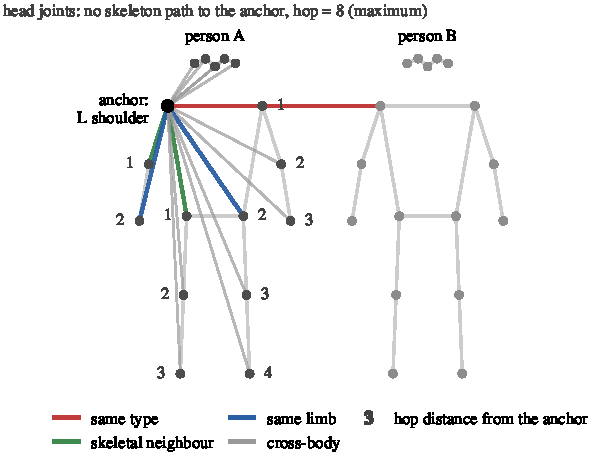
\includegraphics[width=\columnwidth]{figures/edge_categories.pdf}
    \caption{The four edge categories and the skeleton hop distance, drawn from one anchor joint.
    Every edge from the left shoulder of person A is coloured by its category, with the same-type edge
    running to the left shoulder of person B.
    The numbers give the hop distance from the anchor on the sixteen-edge skeleton;
    the head joints have no path to the anchor and take the maximum value.}
    \label{fig:edges}
\end{figure}

\paragraph{Modification 2: skeleton-relative position encoding}
In the baseline, position reaches the attention only through the node features,
and the relative geometry between two connected keypoints must therefore be inferred from the two endpoint representations.
The second modification supplies that geometry directly, adding three features to each edge:
the Euclidean distance $\|\mathbf{p}_i-\mathbf{p}_j\|_2$, the skeleton hop distance $d_{\text{hop}}(t_i,t_j)$
--- the shortest-path distance between the joint types on the skeleton, normalised to $[0,1]$ ---
and a same-type indicator $\mathbb{1}[t_i=t_j]$.
These are concatenated with the category encoding to form the edge descriptor
\begin{equation}
    \mathbf{g}_{ij}
    =
    \left[
        \mathbf{c}_{ij}
        \,\middle\|\,
        \|\mathbf{p}_i-\mathbf{p}_j\|_2
        \,\middle\|\,
        d_{\text{hop}}(t_i,t_j)
        \,\middle\|\,
        \mathbb{1}[t_i=t_j]
    \right]
    \in \mathbb{R}^{7},
    \label{eq:edge_descriptor}
\end{equation}
which passes through the same edge encoder, $\mathbf{e}_{ij}^{\text{geom}} = \phi_{\text{edge}}(\mathbf{g}_{ij})$,
and enters the attention in the same way as Equation~\eqref{eq:pggat_typeattn}.
The hop distance is the most direct description of anatomical structure:
a shoulder and an elbow are one hop apart, a shoulder and an ankle several,
and equal proximity in the image does not carry equal grouping evidence.

\paragraph{Modification 3: same-type repulsion heads}
In a standard layer with $H$ heads, every head attends over the same neighbourhood,
and the signal that separates two left-elbow detections is learned by heads that also model anatomically different
joints.
The third modification reserves capacity for this case.
The layer is split into a standard GATv2 sub-layer with $H_{\text{std}}$ heads over the full neighbourhood $\mathcal{N}(i)$
and a repulsion sub-layer with $H_{\text{rep}}$ heads restricted to same-type edges,
\begin{equation}
    \mathcal{N}_{=}(i)
    =
    \{j \in \mathcal{N}(i) : t_j=t_i\},
    \label{eq:same_type_nbhd}
\end{equation}
with $H_{\text{std}}+H_{\text{rep}}=H$.
The two outputs are concatenated along the head dimension,
\begin{align}
    \mathbf{h}_i^{(l+1)}
    =
    \bigl[\,
        &\mathrm{GATv2Conv}_{\text{std}}
        (\mathbf{h}^{(l)},\mathcal{N}(i))
        \,\big\|\, \nonumber \\
        &\mathrm{GATv2Conv}_{\text{rep}}
        (\mathbf{h}^{(l)},\mathcal{N}_{=}(i))
    \,\bigr],
    \label{eq:pggat_repulsion}
\end{align}
leaving the head count of the layer unchanged.
The repulsion heads see only the comparisons that decide between people of the same joint type,
and the final configuration assigns one of the four heads to this pathway, $H_{\text{rep}}=1$ and $H_{\text{std}}=3$.

\paragraph{Network}
The final PG-GAT has three such layers with four heads and a hidden dimension of 64,
each followed by layer normalisation, a nonlinearity and dropout of 0.1.
A linear projection maps the final representation to the embedding $\mathbf{z}_i \in \mathbb{R}^{256}$,
which is L2-normalised so that every embedding lies on the unit hypersphere.
This bounds the space in which the read-out operates and makes the inner product of two embeddings equal to their cosine
similarity.
These settings were selected by an architecture search rather than inherited from the baseline.

\subsection{Training}
\label{sec:method_training}

% --- from chapter3_baseline.tex 3.5.2-3.5.3 and chapter3_pg_gat.tex 3.8.5 ---
The embedding network is trained with a margin-based contrastive loss~\citep{chopra2005contrastive} on cosine similarity,
$\cos(\mathbf{z}_i,\mathbf{z}_j) = \mathbf{z}_i^\top \mathbf{z}_j$.
Positive pairs $\mathcal{P}^{+}$ contain keypoints of the same person,
$\mathbf{y}^\star_i = \mathbf{y}^\star_j$ with $i \neq j$;
negative pairs $\mathcal{P}^{-}$ contain keypoints of different people.
The objective is
\begin{align}
    \mathcal{L}_{\text{contrastive}}
    =
    &\frac{1}{|\mathcal{P}^{+}|}
    \sum_{(i,j) \in \mathcal{P}^{+}}
    \bigl(
        1 - \cos(\mathbf{z}_i,\mathbf{z}_j)
    \bigr) \nonumber \\
    &+\;
    \frac{1}{|\mathcal{P}^{-}|}
    \sum_{(i,j) \in \mathcal{P}^{-}}
    \max\!\bigl(
        0,\;
        \cos(\mathbf{z}_i,\mathbf{z}_j) - \gamma
    \bigr).
    \label{eq:contrastive_loss}
\end{align}
The first term pulls same-person embeddings towards a cosine similarity of one
and keeps contributing however close they already are.
The second term penalises different-person pairs whose similarity exceeds the margin $\gamma$;
once a negative pair falls below the margin it no longer contributes,
which keeps the gradient on the pairs that are still too close.
The margin is set to $\gamma=0.5$.
For the repulsion heads of Section~\ref{sec:method_pggat}, which see only same-type edges,
the second term is the signal that separates same-type detections of different people.

Training proceeds in two stages.
The network is first trained on 400 procedurally generated synthetic scenes with known person identities,
for 50 epochs at a batch size of 4,
using AdamW~\citep{loshchilov2019adamw} at an initial learning rate of $10^{-3}$ and weight decay $10^{-4}$,
cosine annealing~\citep{loshchilov2017cosineannealing} to $10^{-5}$,
and gradient-norm clipping at 1.0.
The checkpoint with the highest pose grouping accuracy on a held-out synthetic validation split is kept.
It is then fine-tuned on the person-keypoint annotations of COCO \texttt{train2017}~\citep{lin2014coco} under the same
objective, for a smaller number of epochs at a reduced learning rate,
to adapt the embedding to real keypoint statistics while retaining the person-separation structure learned on synthetic
data.
Synthetic pre-training provides exact identities, controlled scene composition and a repeatable setting in
which design changes can be compared without the variation a real detector introduces;
the fine-tuning stage closes the gap to real data.

Apart from the neighbourhood size $k$, the principal hyperparameters of the final model were selected by search rather
than inherited.
Six architectural parameters (number of layers, number of heads, hidden dimension, output dimension,
joint-type embedding dimension and dropout) were selected by a 32-run Bayesian sweep with Hyperband early
termination~\citep{li2018hyperband}, with pose grouping accuracy on the synthetic validation split as the selection
metric; the sweep settled on the three-layer, four-head,
256-dimensional configuration above.
A separate 24-run sweep over the contrastive margin, the number of repulsion heads, the learning rate
and the weight decay returned settings close to the inherited ones, including $\gamma=0.5$,
and the improvement of PG-GAT over the baseline is therefore not a product of retuning the objective.
A further 12-run sweep over the fine-tuning epochs, learning rate and weight decay,
centred on a 20-epoch recipe at $10^{-4}$, selected the 15-epoch schedule.

\subsection{Read-out and person count}
\label{sec:method_readout}

% --- from chapter3_baseline.tex 3.5.3 (read-out) and chapter3_integration.tex 3.12.4 (K estimation), brief per D5 ---
At inference the network is applied once per image to produce the embeddings $\{\mathbf{z}_i\}_{i=1}^{N}$,
which are grouped by $k$-means with $K$ clusters on the unit hypersphere, using ten random initialisations
and a fixed seed~\citep{scikitlearn}.
The read-out is unchanged from the baseline and applies no structural constraint;
PG-GAT changes the representation on which grouping is performed, not the clustering.

When no oracle count is available, $K$ is predicted by a small head, the K-head, trained on the frozen embeddings.
The node embeddings of a scene are summarised by concatenating their mean-pooled
and max-pooled representations with the keypoint count normalised by the seventeen joint types;
a multilayer perceptron maps this vector to a person count and is trained with an L1 loss against the ground-truth
$K$.
Training the head jointly with the embedding network lets the count gradient reach the embedding
and degrades its person separation; the head is therefore trained after the embedding network,
with all embedding parameters frozen.
The final K-head has 35\,009 parameters.
Because keypoint visibility, missing detections and person density differ between synthetic and real data,
the K-head used on COCO is trained on embeddings of COCO \texttt{train2017} scenes, again with PG-GAT frozen.
Two settings are evaluated: oracle $K$, which measures the embedding and read-out alone,
and predicted $\hat K$, which is the complete autonomous pipeline.
\section{Experimental setup}
\label{sec:setup}

\subsection{Datasets}
\label{sec:setup_data}

% --- from chapter3_dataset.tex 3.4.1 ---
\paragraph{Synthetic data}
Because the grouping module never sees the image, its input being a set of keypoint coordinates, joint types
and visibility flags, a rendered scene is as valid a training example as a photograph, provided the geometry of the
keypoints is realistic.
Synthetic scenes also supply labels that annotation cannot.
Every keypoint's position, person identity and visibility follow from the 3D scene,
and a joint hidden behind another person is recorded as present but occluded rather than missing.
The scenes are generated in Blender~\citep{blender}: a configurable number of mannequin meshes is placed, and the
camera, viewing angle, lighting and placement are varied procedurally.
Each scene provides the seventeen COCO keypoints per person with an image position
and a visibility state determined by ray casting against the scene geometry.
The dataset contains 400 training, 100 validation and 100 test scenes.
The number of people per scene is drawn uniformly from $K \in \{1,\dots,5\}$, which gives the grouping network
and the K-head a balanced range of crowding;
the upper limit of five covers the bulk of the target distribution, since
87.5\,\% of the COCO \texttt{val2017} images with keypoint annotations contain five people or fewer.
Depth is available from the renderer but is not used.
With exact depth the standard GATv2 baseline groups synthetic scenes almost perfectly,
0.9990 accuracy on the validation split, yet transfers to COCO worse than without it, 0.8366 against 0.8841,
because real images offer only monocular depth estimates~\citep{ranftl2020midas} of a different scale.
All reported models therefore use the position-and-visibility features of Equation~\eqref{eq:node_feature_no_depth}.

% --- from chapter3_dataset.tex 3.4.2 and chapter3_evaluation.tex 3.13.1 ---
\paragraph{COCO}
Fine-tuning uses the person-keypoint annotations of COCO \texttt{train2017}~\citep{lin2014coco},
approximately 56\,000 images after filtering.
Evaluation uses \texttt{val2017} in three views.
Ground-truth keypoints: the annotated keypoints of the 2\,307 images that form a scoreable grouping instance are
grouped directly, which isolates the grouping network from any detector.
About half of these images contain a single person, for which grouping is trivial;
the 1\,248-image subset with at least two people is therefore reported alongside as the stricter measure.
End-to-end: the annotated keypoints are replaced by detections,
on the 2\,258 images that contain at least one person with three or more visible keypoints;
an image contributes only when at least two detections can be matched to ground truth, which leaves 2\,165, 2\,196
and 2\,121 scored images for HigherHRNet, YOLO11x-pose and RTMO-L respectively.
System-level: all 5\,000 \texttt{val2017} images are used for the average-precision evaluation.

\subsection{Detectors and the joint-trained reference}
\label{sec:setup_detectors}

% --- from chapter3_integration.tex 3.12.1 ---
The primary detector is HigherHRNet-W32 at an input resolution of 512 pixels~\citep{cheng2020higherhrnet,sun2019hrnet},
with its public COCO weights, held frozen throughout.
It is chosen deliberately rather than swapped for a more recent estimator.
Its associative-embedding (AE) grouping~\citep{newell2017associative} predicts a scalar tag at every keypoint,
trained jointly with the heatmaps so that tags of the same person agree and tags of different people separate.
AE is therefore a grouping mechanism learned together with the detector on the COCO training distribution,
with access to the detector's features.
It serves as the joint-trained upper reference:
the comparison measures what is lost when grouping is separated from detection,
not how PG-GAT ranks against the state of the art in pose estimation.
Both groupings receive the same candidate keypoints, extracted by HigherHRNet's own non-maximum suppression,
and their difference is therefore attributable to the grouping stage alone.

% --- from chapter3_integration.tex 3.12.2 ---
The detector swap adds two detectors from different architectural families:
YOLO11x-pose~\citep{ultralytics2024yolo11}, a single-stage model that regresses keypoints per person instance,
and RTMO-L~\citep{lu2024rtmo}, a one-stage bottom-up estimator.
Both return keypoints already assembled into people.
Their person assignments are discarded and all keypoints above a confidence of 0.1 are pooled into one detection set,
the same threshold used for HigherHRNet, before the frozen PG-GAT and the frozen K-head are applied.
No parameter is updated and neither detector contributed training data; the swap is therefore zero-shot.
The discarded assignments are retained and scored as each detector's native grouping on the same matched keypoints.
The RTMO-L weights are the public \texttt{body7} release, trained on a multi-dataset corpus rather than on COCO alone,
which favours its native grouping.

\subsection{Metrics}
\label{sec:setup_metric}

% --- from chapter3_problem_formulation.tex 3.3.4 and chapter3_integration.tex 3.12.3 ---
\paragraph{Pose grouping accuracy}
The primary metric measures the grouping decision alone.
Cluster identifiers produced by $k$-means carry no fixed meaning;
predicted clusters are therefore first aligned with ground-truth people by the Hungarian
algorithm~\citep{kuhn1955hungarian} on their overlap.
With $\pi^\star$ the resulting one-to-one mapping,
pose grouping accuracy (PGA) is the fraction of keypoints assigned to the correct person,
\begin{equation}
    \mathrm{PGA}(\hat{\mathbf{y}}, \mathbf{y}^\star)
    = \frac{1}{N}
      \sum_{i=1}^{N}
      \mathbb{1}\!\left[
          \pi^\star(\hat{\mathbf{y}}_i) = \mathbf{y}^\star_i
      \right],
    \label{eq:pga}
\end{equation}
averaged over images.
On detected keypoints, detections are first matched to annotated keypoints of the same joint type by Hungarian
assignment with a maximum distance of 10 pixels,
and each matched detection inherits the identity of its annotation.
PGA is computed over the matched detections only, for PG-GAT and the native grouping alike,
which excludes detection recall and localisation error and compares the grouping stage on an identical denominator.
In this protocol the graph given to PG-GAT is also built from the matched detections,
and unmatched false-positive keypoints do not enter it.

% --- from chapter4_e2e.tex 4.9.4 and results.md AP@OKS section ---
\paragraph{Average precision}
Published pose estimators are ranked by average precision under the object keypoint similarity (AP@OKS),
which scores complete person instances and is affected by detection failures, localisation error and grouping alike.
A fixed change in PGA has no fixed counterpart in AP;
the two metrics answer different questions ---
PGA isolates the component that PG-GAT replaces, while AP measures the system it becomes part of.
To report the second, the HigherHRNet pipeline is also evaluated with pycocotools on all 5\,000 \texttt{val2017}
images.
In this deployable setting PG-GAT receives every pooled detection above the confidence threshold,
including false positives, and no ground truth enters inference.
Each $k$-means cluster becomes one person instance holding the highest-confidence detection of each joint type,
scored by the mean confidence over the seventeen joint slots.
The native grouping is scored on exactly the same pooled joints, and additionally on its unrestricted output.
The detector wrapper runs single-scale without flip testing, and absolute values therefore sit below
the published 0.671 for this configuration~\citep{cheng2020higherhrnet};
only comparisons within the protocol are meaningful.

\subsection{Implementation}
\label{sec:setup_impl}

% --- from chapter3_baseline.tex 3.5.3 and chapter3_evaluation.tex 3.13.2-3.13.3 ---
The networks are implemented in PyTorch Geometric~\citep{fey2019pyg};
$k$-means uses scikit-learn~\citep{scikitlearn} with ten initialisations and a fixed seed.
Synthetic training selects the checkpoint with the highest pose grouping accuracy on the synthetic validation split, evaluated every five epochs.
The three hyperparameter sweeps use Bayesian optimisation with Hyperband early termination~\citep{li2018hyperband};
the architecture and loss sweeps select on pose grouping accuracy on the synthetic validation split.
Every reported number is linked to a logged run in a Weights \& Biases project~\citep{wandb},
which records the configuration, metric history and checkpoint of the run.
\section{Results}
\label{sec:results}

Results are presented in the order in which they constrain the design: the grouping stage, the embedding network,
adaptation to real data, the end-to-end pipeline and its detector swap, the system-level view,
and the variants that did not improve on PG-GAT.
All values are pose grouping accuracy unless stated otherwise.

\subsection{Grouping heads against the $k$-means read-out}
\label{sec:results_heads}

% --- from chapter4_baseline.tex, chapter4_learned_heads.tex, chapter4_sa_dmon.tex ---
The grouping stage was tested as the bottleneck before any change to the embedding.
Three learned grouping heads were trained jointly with the standard two-layer GATv2 embedding under an identical schedule:
deep embedded clustering (DEC)~\citep{xie2016dec}, slot attention~\citep{locatello2020slotattention}
and supervised graph partitioning~\citep{yang2020gcnve}.
A skeleton-aware deep modularity network (SA-DMoN),
which adds pose structure to a modularity-based clustering objective~\citep{tsitsulin2023dmon},
was trained in ten variants under the same arrangement.
Table~\ref{tab:heads} compares all of them with $k$-means on the same kind of embedding.

\begin{table}[!t]
\centering
\caption{Learned grouping heads against the $k$-means read-out on the standard GATv2 embedding (two layers, $d=128$, synthetic training only).
COCO values use ground-truth keypoints.
``$k$-means'' clusters the embedding trained jointly with each head; ``head'' is the head's own read-out.}
\label{tab:heads}
\footnotesize\setlength{\tabcolsep}{3.5pt}
\begin{tabular}{lccc}
\toprule
Configuration & Synth val & COCO $k$-means & COCO head \\
\midrule
Standard GATv2 + $k$-means & 0.8783 & 0.8841 & --- \\
DEC & 0.8608 & 0.8798 & --- \\
Slot attention & 0.9025 & 0.8254 & 0.7986 \\
Graph partitioning & 0.9714 & 0.8366 & 0.7514 \\
SA-DMoN, 10 variants & 0.777--0.793 & 0.862--0.868 & 0.811--0.821 \\
\bottomrule
\end{tabular}
\end{table}

No head beats $k$-means once the models are scored on COCO.
Slot attention and graph partitioning raise synthetic accuracy, the latter by 0.0931,
but their own read-outs fall to 0.7986 and 0.7514 on COCO,
and $k$-means applied to their jointly trained embeddings still does better than the heads.
DEC leaves the representation largely untouched; its training target is built from its own soft assignments and supplies no identity information.
The ten SA-DMoN variants vary the spatial bandwidth, the null model, the adjacency, and the type loss,
yet all stay inside a 0.0165 band on synthetic data, the best of them 0.0849 below the baseline.
Adding capacity or structure after the embedding does not recover what the embedding lacks, which motivates building the structure into the embedding network itself.

\subsection{PG-GAT ablation and sweeps}
\label{sec:results_ablation}

% --- from chapter4_pggat_ablations.tex and chapter4_pggat_sweep.tex ---
Table~\ref{tab:ablation} isolates the three modifications, all run on the two-layer architecture
and synthetic-only schedule shared with the baseline.

\begin{table}[!t]
\centering
\caption{Isolation ablation of the three PG-GAT modifications at matched architecture (two layers, $d=128$) and training, synthetic training only.
COCO values use ground-truth keypoints.}
\label{tab:ablation}
\footnotesize\setlength{\tabcolsep}{3.5pt}
\begin{tabular}{lcc}
\toprule
Configuration & Synth val & COCO val \\
\midrule
Standard GATv2 (baseline) & 0.8783 & 0.8841 \\
Type-pair attention only & 0.8825 & 0.8819 \\
Position encoding only & 0.8825 & 0.8884 \\
Repulsion heads only & 0.8834 & 0.8785 \\
All three (PG-GAT) & 0.8896 & 0.8868 \\
\bottomrule
\end{tabular}
\end{table}

Each single modification lifts synthetic accuracy by between 0.0042 and 0.0051, and the three together add 0.0113,
a 0.0062 margin over the best single modification.
The single-modification values fall within 0.0009 of one another and are not read as a ranking:
each is a single run, and the individual margins sit close to the metric's run-to-run variation.
Zero-shot transfer to COCO is mixed.
Position encoding alone is the strongest configuration at 0.8884;
type-pair attention and repulsion alone fall slightly below the baseline;
and the full configuration lands 0.0027 above it.
The ablation supports retaining all three modifications but does not assign the later COCO gain to any single one.

The architecture sweep then lifts synthetic accuracy from 0.8896 to 0.9634 ---
a gain of 0.0738, the largest produced by any change to the embedding network ---
by selecting three layers and a 256-dimensional output.
The loss sweep finds no setting above the inherited one; its best run reaches 0.9617.
The benefit of the skeleton-aware modifications depends strongly on the capacity of the network that uses them.

\subsection{COCO fine-tuning}
\label{sec:results_finetune}

% --- from chapter4_coco_ft.tex ---
The architecture-sweep winner, trained on synthetic data only, transfers to COCO at 0.9010 on ground-truth keypoints;
Table~\ref{tab:finetune} records the effect of fine-tuning it on COCO.

\begin{table}[!t]
\centering
\caption{Effect of COCO fine-tuning on the architecture-sweep-selected PG-GAT.
COCO val groups ground-truth keypoints; COCO E2E groups HigherHRNet detections with the annotated person count.}
\label{tab:finetune}
\footnotesize\setlength{\tabcolsep}{3.5pt}
\begin{tabular}{lccc}
\toprule
Configuration & Synth val & COCO val & COCO E2E \\
\midrule
Synthetic only & 0.9634 & 0.9010 & 0.9005 \\
Earlier 20-epoch recipe$^{a}$ & 0.9178 & 0.9565 & 0.9430 \\
Single 20-epoch fine-tune & --- & 0.9695 & 0.9559 \\
Fine-tune sweep (final) & 0.9634 & 0.9715 & 0.9591 \\
\midrule
HigherHRNet AE (reference) & --- & --- & 0.9847 \\
\bottomrule
\end{tabular}

\smallskip
\footnotesize $^{a}$ applied to the two-layer PG-GAT of Table~\ref{tab:ablation}.
\end{table}

Fine-tuning is among the largest effects in the study: COCO accuracy rises by 0.0705 to 0.9715,
and end-to-end accuracy by 0.0586 to 0.9591.
The sweep over the fine-tuning recipe adds only 0.0020 on top of a single fine-tune;
this is not treated as a substantive gain, and its value lies in showing that the result does not depend on one narrowly chosen schedule.
Synthetic accuracy holds at 0.9634, and 0.9580 on the held-out synthetic test split; adaptation to COCO therefore does not come at the cost of the source domain.
On the 1\,248 images with at least two people, the final model reaches 0.9472.

\subsection{End-to-end grouping and detector swap}
\label{sec:results_e2e}

% --- from chapter4_e2e.tex 4.9.1-4.9.3 and 4.9.5 ---
Against the native AE grouping on the same matched HigherHRNet detections,
PG-GAT with the annotated person count reaches 0.9591 against 0.9847, a difference of 0.0256.
That same gap is 0.1081 for the synthetic-only two-layer PG-GAT,
0.0842 for the synthetic-only sweep-selected architecture,
0.0417 for the two-layer PG-GAT under the earlier fine-tuning recipe, and 0.0256 for the final model.
It is not a pure read-out of the cost of modularity: AE and PG-GAT also differ in representation, objective, and access to detector features.
It is, instead, the empirical gap between the modular pipeline and the detector's own grouping under a common protocol.

Swapping the annotated count for the K-head's prediction yields the autonomous pipeline, which consumes no ground truth at inference.
The K-head reproduces the exact annotated count in 76.1\,\% of the 2\,165 scenes and lands within one person in 91.9\,\%.
The autonomous pipeline reaches 0.9644, a 0.0053 margin over the pipeline given the annotated count.
Table~\ref{tab:swap} repeats the evaluation on the two further detectors, applying the same frozen PG-GAT
and K-head with no retraining, and Figure~\ref{fig:swap} shows one scene under all three.

\begin{table*}[!t]
\centering
\caption{Detector swap on COCO \texttt{val2017}.
Recall is the fraction of annotated keypoints matched by a detection within 10 pixels.
Native is each detector's own person assignment on its matched detections; the PG-GAT columns discard it
and re-group the pooled keypoints with the same frozen network,
using the annotated count or the K-head's prediction.
Gap is native minus autonomous PG-GAT; $\hat K$ gain is PG-GAT with $\hat K$ minus PG-GAT with the annotated $K$.
Scored images: 2\,165, 2\,196 and 2\,121.}
\label{tab:swap}
\footnotesize\setlength{\tabcolsep}{3.5pt}
\begin{tabular}{lcccccc}
\toprule
Detector (family) & Recall & Native & PG-GAT, $K$ & PG-GAT, $\hat K$ & Gap & $\hat K$ gain \\
\midrule
HigherHRNet-W32-512 (heatmaps and AE tags) & 0.793 & 0.9847 & 0.9591 & 0.9644 & 0.0203 & $+0.0053$ \\
YOLO11x-pose (single-stage regression) & 0.816 & 0.9863 & 0.9647 & 0.9653 & 0.0210 & $+0.0006$ \\
RTMO-L (one-stage bottom-up)$^{a}$ & 0.774 & 0.9961 & 0.9437 & 0.9741 & 0.0220 & $+0.0304$ \\
\bottomrule
\end{tabular}

\smallskip
\footnotesize $^{a}$ public \texttt{body7} weights, trained on a multi-dataset corpus rather than COCO alone.
\end{table*}

\begin{figure*}[!t]
    \centering
    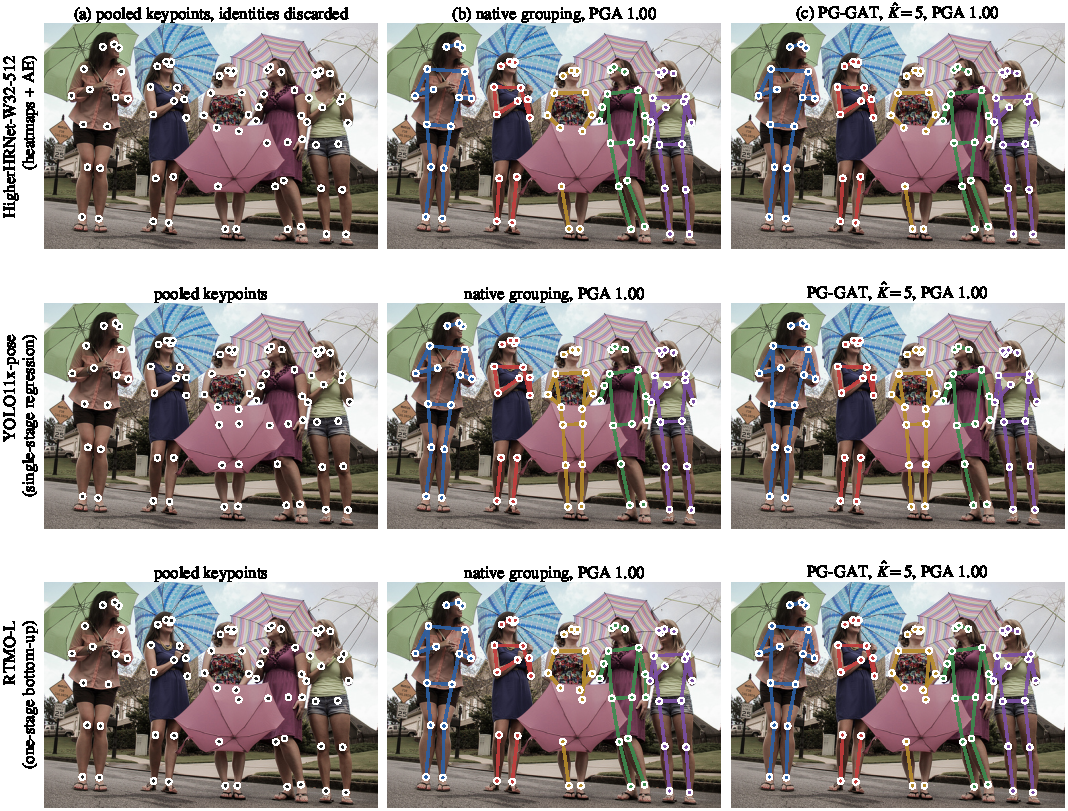
\includegraphics[width=\textwidth]{figures/detector_swap.pdf}
    \caption{One COCO \texttt{val2017} scene (281759, five people) under the three detectors,
    shown to illustrate reuse of the same frozen module rather than a typical error.
    (a) The detected keypoints with the detector's identities discarded, as they cross the interface.
    (b) The detector's native grouping.
    (c) The frozen PG-GAT grouping of all pooled detections with the predicted person count $\hat K$.
    Joints are drawn only where a detection is matched to ground truth and are coloured by the person their group maps to.
    All nine groupings of this scene are correct (accuracy 1.00), so every joint carries its own person's colour.}
    \label{fig:swap}
\end{figure*}

The autonomous pipeline trails the native grouping by 0.0203, 0.0210, and 0.0220 for the three detectors,
a 0.0017 spread across a heatmap-based bottom-up detector, a single-stage regression model,
and a one-stage bottom-up model whose native grouping comes from multi-dataset training.
The accuracy difference between the predicted and annotated counts also shifts systematically with the detector:
the predicted count is worth $+0.0006$ for YOLO11x-pose at a recall of 0.816,
$+0.0053$ for HigherHRNet at 0.793, and $+0.0304$ for RTMO-L at 0.774.
On ground-truth keypoints, where recall is complete, the predicted count instead costs 0.0066 against the annotated count.

\subsection{System-level average precision}
\label{sec:results_ap}

% --- from results.md "AP@OKS end-to-end (2026-09-09)" (not in the dissertation) ---
Table~\ref{tab:ap} scores the same HigherHRNet pipeline under AP@OKS on all 5\,000 \texttt{val2017} images,
with PG-GAT grouping every pooled detection, false positives included.

\begin{table}[!t]
\centering
\caption{AP@OKS on COCO \texttt{val2017} (5\,000 images) for HigherHRNet-W32-512 keypoints, single scale without flip.
All rows except the first group the same pooled joints (confidence above 0.1).}
\label{tab:ap}
\footnotesize\setlength{\tabcolsep}{3.5pt}
\begin{tabular}{lcccc}
\toprule
Grouping & AP & AP$_{50}$ & AP$_{75}$ & AR \\
\midrule
Native, full output & 0.583 & 0.769 & 0.638 & 0.677 \\
Native, pooled joints & 0.540 & 0.749 & 0.579 & 0.630 \\
PG-GAT, predicted $\hat K$ & 0.492 & 0.724 & 0.510 & 0.548 \\
PG-GAT, annotated $K$ & 0.483 & 0.719 & 0.503 & 0.537 \\
PG-GAT, detector's count & 0.484 & 0.713 & 0.503 & 0.539 \\
\bottomrule
\end{tabular}
\end{table}

On identical joints, the autonomous pipeline sits 0.048 AP below the native grouping,
and 0.116 below the native grouping's unrestricted output when both draw on every joint the detector returns (0.583 against 0.467).
The system-level cost is therefore larger than the grouping-level cost of about 0.02 measured on matched detections.
Figure~\ref{fig:crowd} splits both metrics by the number of annotated people.
The AP difference is 0.029 on images with one to five people and 0.076 on images with six or more,
the range beyond the person counts seen in synthetic training.
On matched detections the pose grouping accuracy gap grows in the same way, from 0.016 to 0.053.
At the protocol threshold the predicted count still outperforms the annotated count, 0.492 against 0.483 AP.

\begin{figure}[!t]
    \centering
    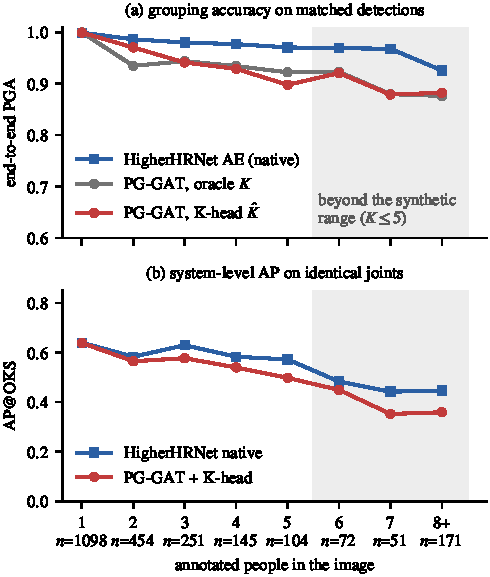
\includegraphics[width=\columnwidth]{figures/crowd_size.pdf}
    \caption{Performance by the number of annotated people in the image, HigherHRNet detections.
    (a) End-to-end pose grouping accuracy on matched detections.
    (b) AP@OKS on identical pooled joints.
    The shaded region lies beyond the person counts of the synthetic training data;
    $n$ is the number of images per bin in (b).}
    \label{fig:crowd}
\end{figure}

\subsection{Variants that did not improve on PG-GAT}
\label{sec:results_variants}

% --- from chapter4_hyperbolic.tex, chapter4_trigat.tex, chapter4_v2.tex ---
Each of three extensions tested a single assumption of the design; Table~\ref{tab:variants} summarises them.

\begin{table}[!t]
\centering
\caption{PG-GAT variants.
COCO val groups ground-truth keypoints; $d$ is the embedding dimension; v2 adds appearance features.}
\label{tab:variants}
\footnotesize\setlength{\tabcolsep}{3.5pt}
\begin{tabular}{lccc}
\toprule
Configuration & $d$ & Synth val & COCO val \\
\midrule
PG-GAT, two layers & 128 & 0.8896 & 0.8868 \\
Hyperbolic PG-GAT & 32 & 0.8856 & 0.8969 \\
TriGAT$^{a}$ & 128 & 0.8740 & 0.8564 \\
\midrule
PG-GAT, final & 256 & 0.9634 & 0.9715 \\
Hyperbolic, COCO fine-tuned & 32 & 0.8900 & 0.9399 \\
PG-GAT v2, 20 epochs & 128 & --- & 0.9670 \\
PG-GAT v2, 50 epochs & 128 & --- & 0.9682 \\
\bottomrule
\end{tabular}

\smallskip
\footnotesize $^{a}$ evaluated on the 2\,180 scenes with at least one valid triplet.
\end{table}

A hyperbolic output space on the Lorentz model~\citep{nickel2018lorentz},
chosen for the tree-like topology of the skeleton,
matches the 128-dimensional Euclidean model at 32 dimensions under synthetic training,
0.8856 against 0.8896.
Fine-tuning removes the advantage: the fine-tuned hyperbolic model reaches 0.9399 on COCO,
0.0316 below the final Euclidean model, and 0.9336 end to end.
TriGAT replaces joints with triplets of connected joints --- the pivot angle of a triplet describing local articulation independently of rotation ---
and votes the triplet clusters back onto joints; it lands 0.0156 below the matched PG-GAT on synthetic data
and 0.0304 below on COCO, with the loss traced to the voting stage.
PG-GAT v2 adds MobileNetV2 features~\citep{sandler2018mobilenetv2} sampled at each keypoint; it stays 0.0045
and 0.0033 below the final model while adding a further $2.2 \times 10^{6}$ frozen parameters at inference.
Because it extends the earlier two-layer architecture, it does not isolate the effect of appearance on the final configuration.
None of the three is a better operating point than the position-and-type PG-GAT.
\section{Discussion}
\label{sec:discussion}

\subsection{The embedding is the lever}
\label{sec:disc_embedding}

% --- from chapter5_embedding.tex 5.1.1-5.1.4 ---
Section~\ref{sec:results_heads} and Section~\ref{sec:results_ablation} point the same way.
The three learned heads and the ten modularity variants all add capacity or structure after the embedding,
and none improves on $k$-means once the model meets real data; in several cases, $k$-means on a head's own jointly
trained embedding does better than the head.
The failures have distinct causes: DEC sharpens its own assignments without introducing any new identity
information, slot attention carries no notion that two joints of the same type must belong to different people,
and graph partitioning turns small shifts in pairwise affinity into changes in connected components.
The modularity variants all plateau, since the $k$NN graph encodes proximity rather than identity,
and none of the ten reformulations of the objective recovered identity communities from it.
Changing the embedding, by contrast, is what produces the only gains that survive transfer --- a small one from the
three skeleton-aware modifications at matched capacity, and larger ones from the architecture sweep stacked on top
of them and from fine-tuning on COCO.
Within the grouping methods evaluated here, additional complexity at the read-out contributes less than improving the
representation it receives, and once the embedding separates people well a simple read-out is adequate.

Figure~\ref{fig:embedding} shows what this means for a single scene.
Chosen from the 180 COCO scenes with three to five people and at least ten annotated keypoints per person,
it is the one whose per-scene pose grouping accuracy under the three checkpoints lies closest to the dataset-level
accuracy, making it representative rather than chosen for effect.
The standard GATv2 embedding places several keypoints of one person inside another person's cluster, four of them
misassigned; the synthetic-only PG-GAT cuts this to three; and the fine-tuned PG-GAT collapses each person to a tight
cluster, misassigning none.
The similarity matrices show the same progression without a projection: the within-person block structure sharpens,
and cross-person similarity becomes uniform.

\begin{figure*}[!t]
    \centering
    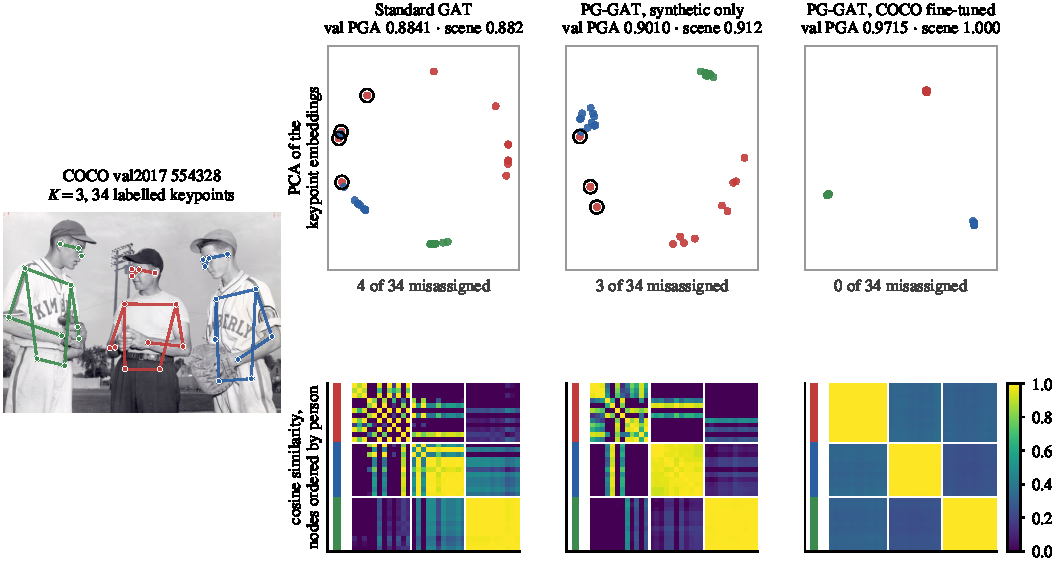
\includegraphics[width=\textwidth]{figures/embedding_space_pca.pdf}
    \caption{The embedding of one COCO \texttt{val2017} scene (554328, three people, 34 annotated keypoints) under three checkpoints: the standard GATv2 baseline, PG-GAT after synthetic training, and PG-GAT after COCO fine-tuning.
    Top: principal-component projection of the keypoint embeddings, coloured by person;
    keypoints the $k$-means read-out assigns to the wrong person are ringed.
    Bottom: cosine similarity between the keypoint embeddings, ordered by person.
    Column titles give the dataset-level pose grouping accuracy on COCO and the pose grouping accuracy on this scene.}
    \label{fig:embedding}
\end{figure*}

The attention itself shows where the modifications act (Figure~\ref{fig:attention}).
Across the 1\,248 multi-person validation scenes, the standard heads of PG-GAT place less than 0.001 of their attention
on same-type edges --- against 0.041 for uniform attention over the neighbourhood --- and 0.292 on skeletal-neighbour
edges, against a uniform share of 0.173.
The share of attention that stays within a person rises through the three layers, from 0.74 to 0.90 and 0.93, whereas in
the baseline it is 0.765 against a uniform 0.717.
The edge categories therefore let PG-GAT route information along the skeleton of the correct person.
The baseline here is the synthetic-only two-layer model, and the comparison with it accordingly reflects the complete
final model rather than the three modifications alone; the comparison of each model with uniform attention does not
depend on this.
The dedicated repulsion head places 0.675 of its attention on the node itself, against 0.589 under uniform attention,
and 0.325 on same-type neighbours, against 0.411; it therefore passes a node's own representation through more than
it compares same-type neighbours.

\begin{figure*}[!t]
    \centering
    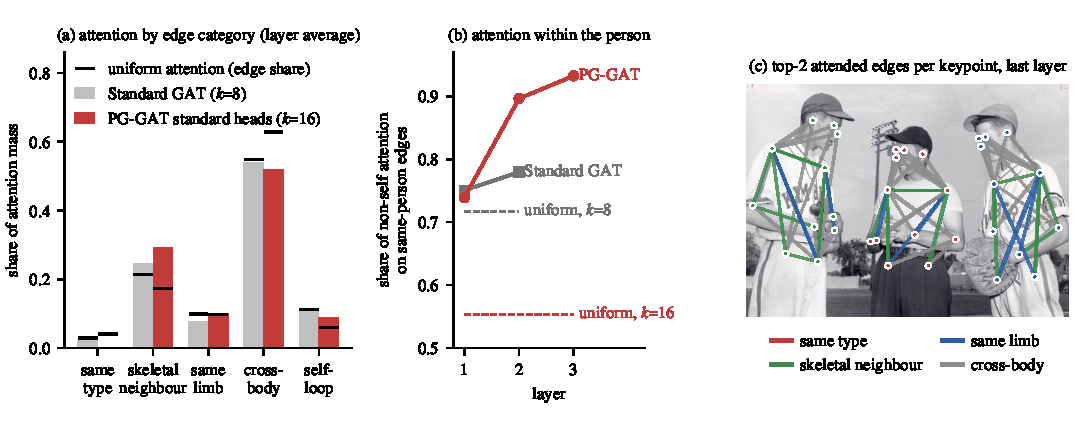
\includegraphics[width=\textwidth]{figures/attention_edges.pdf}
    \caption{Attention of the standard GATv2 baseline and of PG-GAT's standard heads over the 1\,248 multi-person COCO \texttt{val2017} scenes.
    (a) Share of attention by edge category, averaged over layers;
    black ticks mark the share that uniform attention over the neighbourhood would give.
    (b) Share of attention on edges within the same person, per layer, with the uniform share dashed.
    (c) The two most-attended incoming edges of every keypoint in the final layer on the scene of Figure~\ref{fig:embedding},
    coloured by category.}
    \label{fig:attention}
\end{figure*}

\subsection{What survives synthetic-to-real transfer}
\label{sec:disc_transfer}

% --- from chapter5_transfer.tex 5.2.1-5.2.6 ---
Throughout, synthetic accuracy was a poor predictor of real accuracy.
Exact depth made synthetic grouping almost perfect and real grouping worse; graph partitioning was the best synthetic
head and among the worst on COCO; the hyperbolic embedding matched a Euclidean one of four times its dimension on
synthetic data but not after fine-tuning; and fine-tuning itself, which changes no part of the architecture, yielded a
gain of 0.0705 on COCO, comparable in size to the 0.0738 that the whole architecture sweep added on synthetic data.
Figure~\ref{fig:transfer} plots this pattern across all 27 configurations that carry both measurements.
Synthetic training remains valuable as a controlled setting with exact identities in which architectural ideas can be
isolated, and as the starting representation that fine-tuning then adapts; an improvement measured there counts as
evidence only when the mechanism behind it also makes sense on real keypoints.
The variants of Section~\ref{sec:results_variants} illustrate the point: each introduced structure motivated in
principle, and none produced an advantage at the COCO operating point.

\begin{figure}[!t]
    \centering
    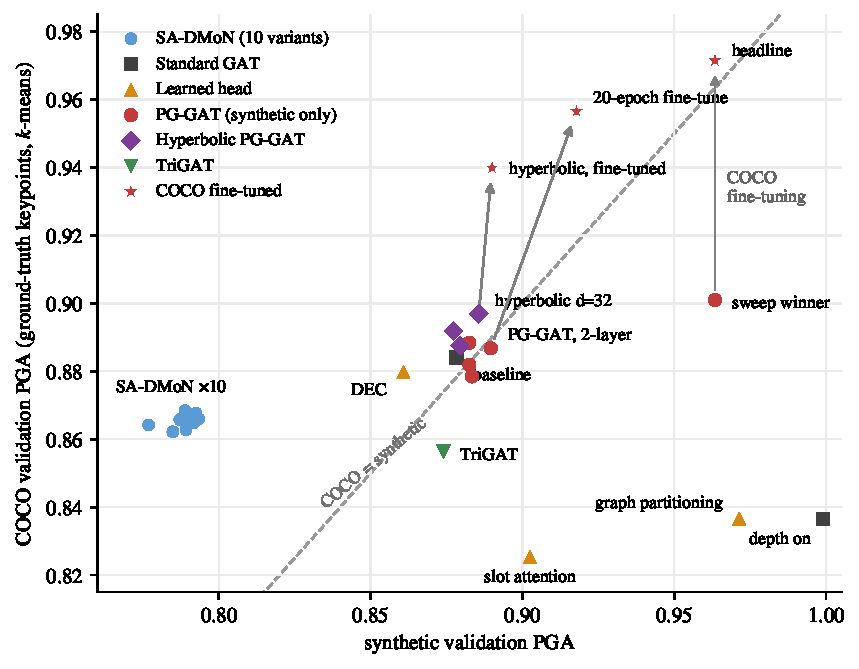
\includegraphics[width=\columnwidth]{figures/transfer_scatter.pdf}
    \caption{Synthetic-validation pose grouping accuracy against COCO-validation pose grouping accuracy on ground-truth keypoints, for the 27 configurations that report both.
    Points below the diagonal lose accuracy in transfer;
    arrows join the synthetic-only models to their COCO fine-tuned versions.}
    \label{fig:transfer}
\end{figure}

\subsection{The cost of modularity and the effective person count}
\label{sec:disc_modularity}

% --- from chapter5_modularity_autonomy.tex 5.3.1-5.3.3; effective-K numbers from results.md per-image dump ---
Separating grouping from detection carries a measured cost.
On matched detections the autonomous pipeline trails the native grouping by 0.0203 to 0.0220 across the three detector
families, and the stability of that difference suggests it belongs to the modular formulation rather than to an
interaction with one detector.
The likely source is information the native mechanisms have and PG-GAT does not: AE tags are learned together with the
detector's features and training distribution, whereas PG-GAT sees only coordinates, visibilities, and joint types.
Nor is modularity bought through a smaller model; PG-GAT has 333\,552 parameters, against about 561 in HigherHRNet's tag
head within a detector of 28.6 million.
What the cost buys is reuse --- the same frozen network groups the output of three different detectors without
retraining, which the native mechanisms, embedded in their own detectors, do not offer.
For a fixed detector whose native grouping is available, the results favour the native grouping; the modular design is
useful where detectors are exchanged, upgraded, or developed independently of the grouping stage.
The system-level measurement sharpens the point: on identical joints the cost is 0.048 AP, rising to 0.076 in scenes with
six or more people, beyond the synthetic training range (Section~\ref{sec:results_ap}), and the matched-detection
accuracy therefore understates what a deployed system loses.

The K-head behaves unexpectedly.
Replacing the annotated count with an estimate might be expected to add error, yet on HigherHRNet detections it raises
accuracy by 0.0053 even though it matches the annotated count in only 76.1\,\% of scenes.
The annotated count describes the people in the image, whereas $k$-means operates on the detections that survive; at a
keypoint recall of 79.3\,\%, some annotated people contribute few or no detections, and forcing a cluster for them
splits a well-represented person instead.
The head predicts from the detected embeddings and their number; its mean prediction of 2.46 people sits below the
annotated mean of 2.74.
Measured against the number of distinct annotated people actually present among the matched detections, its exact
agreement rises from 76.0\,\% to 82.1\,\% in a re-run of the evaluation.
The detector swap supports this reading (Figure~\ref{fig:predk}): the advantage of the predicted count grows as recall
falls and reverses sign once the input is complete.
The four points are consistent with an effective-person-count mechanism rather than proof of it, since detector
identity, visibility patterns, and localisation also differ between them.
In a modular pipeline behind an imperfect detector, estimating the count from the detections is therefore not merely a
stand-in for an oracle; the annotated count is not necessarily the right target for the input the grouping stage
actually receives.

\begin{figure}[!t]
    \centering
    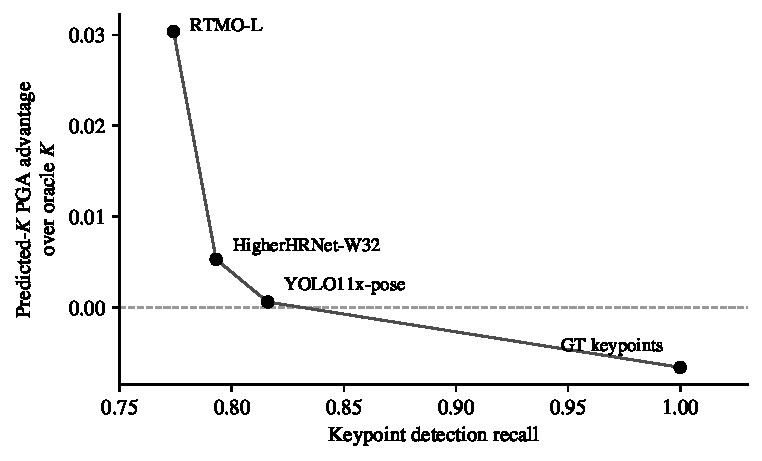
\includegraphics[width=\columnwidth]{figures/predk_recall.pdf}
    \caption{Difference in end-to-end pose grouping accuracy between the predicted and the annotated person count, against keypoint recall, for the three detectors and for ground-truth keypoints.}
    \label{fig:predk}
\end{figure}
\section{Limitations}
\label{sec:limitations}

\paragraph{Crowded scenes}
Synthetic pre-training spans one to five people.
COCO fine-tuning and the K-head do encounter larger scenes, but such scenes form a minority:
12.5\,\% of the \texttt{val2017} images with keypoint annotations contain six or more people.
On those images the K-head predicts the exact count in 22.9\,\% of scenes
and under-counts in 69.4\,\%, and the AP gap to the native grouping widens from 0.029 to 0.076.
Extending the person-count range of the synthetic data is one direct remedy.

\paragraph{Pose grouping accuracy and system accuracy}
The primary metric scores the grouping of matched detections,
and in that protocol the graph handed to PG-GAT is likewise built from matched detections;
false-positive keypoints therefore never reach it.
The system-level AP evaluation lifts both restrictions
and shows a larger cost than the matched-detection accuracy suggests.
PGA remains the right instrument for locating the bottleneck in the grouping stage,
but it is not an estimate of deployed performance.

\paragraph{Extremities and the skeleton prior}
On multi-person scenes the misassignment rate of PG-GAT with the annotated count rises from 5--6\,\% at the shoulders to 10.6--12.1\,\% at the ankles,
while the native grouping stays within 2.6\,\% to 4.4\,\% for every joint type.
The skeleton that supplies the edge categories and hop distances omits the links between the head and the shoulders;
head joints are nevertheless grouped more accurately than body joints,
and the omission therefore does not explain the deficit.
Structure beyond individual joints, such as limbs, is not represented in the model.

\paragraph{Single runs}
The ablation, the sweeps, and the variants are single training runs,
with no repeated seeds or confidence intervals.
Differences of the size of the individual modification gains, or of the 0.0020 fine-tuning-sweep improvement,
are not established as systematic.
The graph's neighbourhood size was left out of every sweep.

\paragraph{Detector comparisons}
The matched subsets differ in size and recall from one detector to another,
and accuracies are comparable within a detector but only with caution across detectors.
The RTMO-L native grouping draws on weights trained over a multi-dataset corpus.
The AP evaluation runs a single-scale HigherHRNet wrapper without flip testing,
and its absolute values fall below the detector's published figure.
\section{Conclusion}
\label{sec:conclusion}

This work separated multi-person pose grouping from keypoint detection and measured what the separation costs.
PG-GAT --- a graph attention network with a type-pair attention bias, skeleton-relative position encoding,
and same-type repulsion heads --- embeds the detected keypoints so that a plain $k$-means read-out recovers the people.
Trained on synthetic scenes and fine-tuned on COCO,
it reaches a pose grouping accuracy of 0.9715 on ground-truth keypoints and 0.9591 on HigherHRNet detections,
against 0.9847 for the detector's own jointly trained grouping.
With a K-head trained on the frozen embeddings, the pipeline runs with no ground truth at inference,
and the same frozen network, applied zero-shot to YOLO11x-pose and RTMO-L, trails each detector's native grouping by about 0.02.
The cost is larger at the system level, 0.048 AP on identical joints, and it concentrates in crowded scenes.
Across the study, changes to the embedding moved accuracy far more than changes to the grouping stage:
learned heads and modularity-based clustering did not improve on $k$-means, while the skeleton-aware attention,
the architecture it was sized to, and fine-tuning on real data did.

The results point to three directions.
Extending the synthetic data beyond five people addresses the largest measured deficit,
and representing structure above the joint, so that a wrist is disambiguated through its limb,
targets the errors that concentrate at the extremities.
Repeating the key comparisons over multiple seeds would establish
which of the smaller differences reported here are systematic.
% AGENT DRAFT - Dean to rewrite (D12, 2026-09-28). CVIU requirements: paper_cviu/cviu_author_guide_facts.md items 10, 11, 17.
% Bracketed items are placeholders only Dean can fill: what is released and where. CRediT roles go into the submission system (guide D13); Acknowledgements removed (feedback round 1, item 11).
\section*{Declaration of competing interest}
The authors declare that they have no known competing financial interests or personal relationships that could have appeared to influence the work reported in this paper.

\section*{Data availability}
The synthetic dataset, the code and the trained checkpoints [will be made available at: repository link].
Every reported result is linked to a logged run in the Weights \& Biases project \texttt{multiperson-pose-grouping} [public link].
COCO is publicly available.

\section*{Declaration of generative AI and AI-assisted technologies in the manuscript preparation process}
During the preparation of this work the authors used Claude (Anthropic) to find and summarise candidate references,
to write parts of the research code, evaluation scripts and figure scripts,
to produce a first draft of the manuscript from the experimental record, and to check the numerical
and factual consistency of the text against the logged results.
Every cited work was checked against its source, and the manuscript was rewritten by the authors.
After using this tool, the authors reviewed and edited the content as needed
and take full responsibility for the content of the publication.


%% Bibliography: paper.bib = the 46 cited entries copied from the dissertation's verified file (via the symlink diss_thesis.bib), plus the DOIs found on Crossref (guide D14).
%% A newly cited entry goes into paper.bib, not into the dissertation's file.
\bibliographystyle{model2-names}
\bibliography{paper}

\end{document}
